%                                                                 aa.dem
% AA vers. 9.1, LaTeX class for Astronomy & Astrophysics
% demonstration file
%                                                       (c) EDP Sciences
%-----------------------------------------------------------------------
%
%\documentclass[referee]{aa} % for a referee version
%\documentclass[onecolumn]{aa} % for a paper on 1 column  
%\documentclass[longauth]{aa} % for the long lists of affiliations 
%\documentclass[letter]{aa} % for the letters 
%\documentclass[bibyear]{aa} % if the references are not structured 
%                              according to the author-year natbib style

%
\documentclass{aa}  

%
\usepackage{graphicx}
\usepackage{ulem}
%%%%%%%%%%%%%%%%%%%%%%%%%%%%%%%%%%%%%%%%
\usepackage{txfonts}
\usepackage{todonotes}
\newcommand{\TD}[1]{\textcolor{magenta}{\bf [To do] #1}}
%%%%%%%%%%%%%%%%%%%%%%%%%%%%%%%%%%%%%%%%
\usepackage{xcolor}
\usepackage[hyperref]{hyperref}
% To add links in your PDF file, use the package "hyperref"
% with options according to your LaTeX or PDFLaTeX drivers.
%

\begin{document} 

  \title{Detection of long period exoplanets by gravitational waves}


  \author{Marcus Haberland
            \inst{1}\fnmsep\thanks{marcush@ethz.ch}
          \and
           Lavinia Heisenberg\inst{1}
           \and
          Prasenjit Saha
          \inst{2}
           \and
           Deniz Soyuer
          \inst{3}
          \and
          Lorenz Zwick
          \inst{3}
          }

  \institute{Institute for Theoretical Physics, ETH Zurich, Wolfgang-Pauli-Strasse 27, CH-8093 Zurich\\
         \and
         Physik-Institut, Universit{\"a}t Z{\"u}rich, Winterthurerstrasse 190, CH-8057 Z{\"u}rich, Switzerland\\
         \and
           Center for Theoretical Astrophysics and Cosmology, Institute for Computational Science, University of Zurich, Winterthurerstrasse 190, CH-8057 Zurich
             }

  \date{Received XXXX XX, 2021; accepted XXXX XX, 2021}


%   \date{Received September 15, 1996; accepted March 16, 1997}

% \abstract{}{}{}{}{} 
% 5 {} token are mandatory
 
  \abstract
  % context heading (optional)
  % {} leave it empty if necessary  
   {Past years have seen the investigation of a novel exoplanet detection method for planets around gravitational wave (GW) emitting binary star systems, with the help of the Laser Interferometer Space Antenna (LISA). The suggested technique is conceptually similar to that of radial velocity measurements, where the orbital motion of an exoplanet induces a detectable Doppler shift in the GW frequency. Coincidentally, the significance of missions to Uranus and Neptune have been underlined in the past years by numerous publications. Proposed mission plans usually involve a $\sim 10$ year cruise time to the ice giants. }
  % aims heading (mandatory)
   {This cruise time, which would be concurrent to the LISA mission, can be utilized to search for low-frequency GWs by observing the Doppler shift caused by them in the Earth-spacecraft radio link. As the maximum recoverable orbital period of the imprint of exoplanets in GWs is related to the nominal mission lifetime, we investigate the potential of ice giant missions to detect long period Jupiter’s around binary star systems. }
  % methods heading (mandatory)
   {We calculate the GW strain in an ice giant mission, review the Fisher information analysis for LISA, and utilize it to compute the uncertainties of exoplanet periods and minimum masses recovered with this method.}
  % results heading (mandatory)
   {We find that for an ice giant mission which is at least $1\%$ as sensitive as LISA for some binary systems, a joint search may enable the discovery of circumbinary partners with orbital periods of 10 years or more, raising the upper bound by an order of magnitude compared to LISA on its own.}
  % conclusions heading (optional), leave it empty if necessary 
   {}

   \keywords{Gravitational waves -- white dwarfs -- binaries -- Planets and satellites: detection -- Planets and satellites: individual: Uranus --
                Planets and satellites: individual: Neptune
               }

   \maketitle
%
%-------------------------------------------------------------------

\section{Introduction}

% Background exoplanets
The progress in exoplanet detection over the last twenty years is astonishing, with close to 5'000 exoplanets having been confirmed via electromagnetic (EM) techniques, mainly transit, radial velocity (RV) measurements, micro-lensing and direct imaging \citep{Exo_NASA}. And although we have already learned a lot about exoplanets, their properties, formation and migration processes outside of our own solar system through these means, each detection channel comes with it's own biases and tragically remains mostly blind to more exotic systems, such as exoplanets around white dwarfs (WDs) and binary double WDs (DWDs). 

% Background WDs and DWDs
Only two exoplanets around WDs have been confirmed as of now \citep{vanderburg2020,luhman2011,Exo_NASA}, and none around DWDs \citep{tamanini}, owing mainly to their intrinsic faintness, which hinders EM observations. This proves however, that planets can either survive their host-stars evolution, as further suggested by past theoretical work \citep{duncan1998}, or may be captured after the host's red giant and/or asymptotic giant branch phase. Furthermore, as $\sim 97\%$ of stars will end their lives as WDs \citep{althaus2010}, and around 50\% of Solar-type stars are not single \citep{duchene2013}, we would expect a considerable population of DWDs in the Milky Way alone. If any of them harbor P-type exoplanets, which have been detected around similar systems such as e.g. NN Ser, containing a WD and a millisecond pulsar \citep{beuermann2011}, their detection would give us new insights into if and how planets may survive one or more common-envelope phases.

% Background GW astronomy
On a similar note, multimessenger astronomy has emerged in the last years with the goal in mind, that a combination of different measurement techniques reduces systematic error sources, and results in a higher scientific yield, due to different parameters being recoverable. Since the first gravitational wave (GW) detection, namely GW150914 \citep{abbott2016}, the era of GW astronomy has begun. The launch of the Laser-Interferometer Space Antannae (LISA) currently planned for 2037, is therefore highly anticipated, as LISA will be sensitive to GWs in the so-far unprobed millihertz regime, opening a new window to our galaxy and the universe. 

\section{Detectors}
\subsection{Space-borne Interferometers} \label{sec:spaceborne}
% DWD CBPs in LISA / Taji
As DWDs with orbital periods $T < 1$ h would emit nearly monochromatic GWs in LISA's sensitive frequency range, around $26\times 10^3$ detached DWDs should be resolved by a four year LISA mission \citep{danielski}. This stands in contrast to the current sample of $\sim 150$ DWDs with known orbital parameters \citep{korol2022}, which indicates the possibility to look for exoplanets around them not via EM, but GW techniques, as extensively illustrated by \citep{tamanini,danielski,kang2021}. The proposed method for LISA is conceptually similar to RV in EM observations, but with the DWD GW signal as the carrier wave instead of the host-star's light and is reviewed in Sec. \ref{sec:LISA}. To current consensus between 3 and 83 exoplanets and an order of magnitude more brown dwarfs (BDs) may be detectable around DWDs with this method by LISA on it's own, if one assumes a 50\% occurrence rate for circumbinary exoplanets (CBPs), as hinted at by WD pollution studies \citep{danielski,kang2021}. This is already very promising, as we may find the first exoplanets around DWDs and learn about their occurances and parameter distributions, but leaves room for improvement.

% Problem
The problem in this detection method is three-fold: a) One needs high signal-to-noise ratios $S/N \gg 1$ of the DWD in order to observe the signal of an exoplanet in the first place, strongly reducing the number of promising systems. b) As with classical RV techniques, this method is strongly biased to favor massive planets with orbital periods $P$ comparable to the nominal mission life-time, in LISA's case four years, which have close to coplanar orbits with the line-of-sight (LOS). c) As space-borne missions orbit the sun next to earth, planets with periods comparable to a multiple of one year can't be resolved because of a high correlation with the doppler shift due to the detectors orbit. In this work, we want to investigate a novel possibility in tackling all of these problems with the addition of a spacecraft doppler tracking search.

\begin{figure}[h]
    \centering
    \includegraphics[width=.5\textwidth]{exoplanets.pdf}
    \caption{Confirmed exoplanets with measured or estimated mass and orbital period and their means of detection. Note the scarcity of Jupiter like planets, i.e. planets with $M_P\approx M_J$ and $P \approx 12$ yr. We used data from the \href{https://exoplanetarchive.ipac.caltech.edu/}{NASA Exoplanet Archive}.}
    \label{fig:geometry}
\end{figure}

\subsection{Doppler tracking by future missions to Uranus and Neptune}

%\TD{Swiper no swiping - please rephrase}

Over the past years, a number of white papers have been calling for missions to the ice giants Uranus and Neptune \citep{simon2020,abigail,whitepaper,whitepaper2,whitepaper3}. The scientific potential of possible missions, along with various mission designs have also been extensively discussed in \citep{hofstadter,fletcher,fletcher2,helled,quest,simon2020,kollmann}. Such missions are destined to spend most of their time in interplanetary space, rather than orbiting their respective planets, which reduces the science potential of such missions to a fraction of their life time. If the transponders on these spacecrafts were however used to detect GWs via Doppler tracking during the cruise phase, these missions would also offer a unique (and $\it{cheap}$) opportunity to look for low-frequency GWs. This was previously illustrated by \citep{soyuer2021}.

Additionally, a consensus is being reached in the community regarding the launch date of a possible ice giants mission that would maximize the payload and consequently have a high science yield. The time frame is reported to be around 2029-2030 for Neptune and early 2030s for Uranus, especially if a Jupiter Gravity Assist will be used to reach the ice giants \citep{hofstadter}, which would enable an ice giant mission to run in parallel with LISA and potentially Taiji, a planned space-borne interferometer of the Chinese space agency similar to LISA. By performing a joint search, we expect to raise the global $S/N$ of loud DWDs, raise the maximum $P_{max}$ up to the nominal life-time of an ice giant mission of ten years, and help differentiate exoplanets with a period close to a multiple of one year, due to no earth-like orbit of ice giant missions.

% \TD{paragraph about recent peaking interest in ice giant missions}

% \TD{cite millions of papers}

%\TD{shortcomings of most popular exoplanet detection methods and why they cant detect long period planets that easily}

%\TD{maybe a plot of detected exoplanets showing the gap in long period regime}

\section{Methods}
\label{sec:met}

We followed up with our analysis on \citep{tamanini} and the Fisher information approach as discussed by \citep{cutler}. We first reproduced the analysis of Tamanini for LISA and then translated the idea to the Doppler tracking survey with the help of \citep{armstrong}. We review the Fisher information approach in Sec. \ref{sec:Fisher} and show the derivation for the translated approach to an ice giant mission in Sec. \ref{sec:IG}.

If a DWD system of masses $M_1,\ M_2$ orbits with orbital period $T$ shorter than 1 h, it emits nearly monochromatic GWs with frequency twice the orbital frequency $f_0=\frac{2}{T}$ in LISA's frequency band. Due to the decay of eccentricity via the emission of GWs, we expect rather circular orbits and note, that for more rare high eccentricity orbits, the system would emit a discrete spectrum of waves. 

\begin{figure}[h]
    \centering
    \includegraphics[width=.45\textwidth]{Geometry_Exoplanet.png}
    \caption{Geometric setup of a DWD-CBP three-body system. The angular momentum of the orbits are highlighted for the CBP at the total CoM with inclination $i$, and for the DWD at their CoM with inclination $i_b$ towards the line of sight.}
    \label{fig:geometry}
\end{figure}

The addition of a P-type circumbinary planet (CBP) with mass $M_P$ and orbital period $P \gg T$ results in a Keplerian orbit of the CBP and DWD around the total centre of mass (CoM). Through the Doppler effect, the induced radial velocity of the DWD along the line of sight (LoS) yields a shift in frequency, that in principle can be resolved by GW measurements. We treat the three-body system due to assumed large separation between the DWD and CBP as two separate two-body problems, and further utilize the same simplifications as \citep{tamanini}, namely circular orbits of the DWD and CBP, as well as the radial motion of the DWD being perturbed by only one, dominating CBP. By defining the DWD mass $M_b = M_1 + M_2$, and the initial angle of the motion $\varphi_0$, one finds with the planets inclination as in Fig. \ref{fig:geometry} a radial velocity of the DWD system of

\begin{equation}
    v_{r,b} = -cK\cos{\left(\frac{2\pi}{P}t + \varphi_0\right)}
\end{equation}

where we defined the parameter

\begin{equation}
cK = \frac{2\pi G}{P}^{1/3} \frac{M_P}{(M_b + M_P)^{2/3}}\sin{i}.
\end{equation}

In the DWD reference frame, it emits nearly monochromatic radiation with frequency $f=f_{0} + f_1 t$, where we added the decay of the orbit of the DWD due to emission of gravitational radiation via

\begin{equation}
    f_1=\Dot{f}(t=0)= \frac{96}{5}\pi^{8/3}f_0^{11/3}\left(\frac{GM_c}{c^3}\right)^{5/3}
\end{equation}

with $M_c$ the DWD chirping mass. We stop the taylor series at second order, as for typical DWDs detectable in LISA we already expect $f_0/f_1 \gtrsim 10 $ yr. Now, due to the induced radial velocity of the binary, we find a GW with frequency

\begin{equation} \label{eq:freq}
f_{\text{obs}}= \left(1+\frac{v_{r,b}(t)}{c}\right)f=\left(f_{0} + f_1 t\right) \left(1-K\cos{\left(\frac{2\pi}{P}t + \varphi_0\right)} \right).
\end{equation}    

Finally, this results in a phase of the GW of

\begin{equation} \label{eq:phase}
\begin{split}
\Psi_{\text{obs}}(t) &= 2\pi\int_0^{t}f(t')dt' + \Psi_0 \\
 &= \frac{2}{4\pi} \Bigg( K P \bigg(2 \pi 
   f_0 \sin (\varphi_0) -2 \pi  (f_0+f_1 t) \sin \bigg( \frac{2 \pi  t}{P}+\varphi_0\bigg) \\
   &- f_1 P \cos \left(\frac{2 \pi  t}{P}+\varphi_0\right)+f_1 P \cos (\varphi_0)\bigg) \\
   &+ 2 \pi^2 t (2 f_0+f_1 t) \Bigg) + \Psi_0.
\end{split}
\end{equation}

Dependant on the given detector geometry, this GW will result in a signal $h(t)$ which can be investigated in real data via matched filtering. In this procedure, the noisy signal is compared to a variety of simulated signals in order to claim detection and determine the relevant parameters of the GW source with some uncertainty. 

For a DWD, the relevant parameters are: The amplitude of the GW, $\mathrm{ln}(A)$; the position of the source in heliocentric ecliptic coordinates $\theta_S$ and $\phi_S$; the polarization of the GW due to the relative orientation of the orbital plane, characterised by the angular momentum $\hat{L}_b$ as in Fig. \ref{fig:geometry}, or again in heliocentric ecliptic coordinates by the two angles $\theta_L$ and $\phi_L$; the frequency of the GW specified through $f_0$ and $f_1$; as well as the initial phase $\Psi_0$.  We will however omit $\Psi_0$ as a parameter of the GW in our analysis, to reduce the computational cost and as there is little information lost with the initial phase. With the measurement of these 6 quantities we can additionally infer the distance of the DWD to us, and the masses and separation of the two WDs.

If we introduce CBPs around these kinds of system, we are additionally interested in the orbital period $P$ of the CBP, as well as its minimal mass $M_P\sin (i)$, connected to $K$ as defined above, and the initial phase of the CBP $\varphi_0$. This results in a total of 9 parameters of interest for a given DWD-CBP system. From now on, we will label those parameters as $\lambda=\big(\lambda_i\big)_{i=1}^{9}$.

To estimate the uncertainty of a recovered parameter in advance, we employ the Fisher information approach as described by \citep{cutler} for LISA.

\subsection{Signal analysis}
\label{sec:Fisher}

As a short review, assume we know the expected signal of a source in dependence of all the parameters, $h(t;\lambda)=\mathbf{h}(\lambda)$. Then the measured signal of our detector will be a time series $s(t)=\mathbf{s}$, and in particular a sum of different GW signals as well as a noise realization $n(t)=\mathbf{n}$, which we assume to be Gaussian and stationary.

Stationarity refers to the assumption, that different fourier components of the noise $\Tilde{n}(f)$ are uncorrelated

\begin{equation}
\langle \Tilde{n}(f) \Tilde{n}(f')^* \rangle = \frac{1}{2} \delta (f-f') S_n(f)
\end{equation}    
where the brackets $\langle \dots \rangle$ refer to the ensemble average of the noise over many realizations of the system, and $S_n(f)$ is called the \textit{single-sided noise spectral density} of our detector. It is related to the total variance of the noise as $\langle n^2(t) \rangle=\int^\infty_0 S_n(f)df$ and can be interpreted as the time-averaged variance of the noise at a given frequency.

Gaussianity on the other hand refers to the probability density function (pdf) for a single realization of noise. By introducing the scalar product

\begin{equation} \label{eq:innerprod}
\big(\, \mathbf{j}\,|\,\mathbf{k}\,\big)=2\mathrm{Re}\int^\infty_{-\infty} df\frac{\Tilde{j}^*(f)\Tilde{k}(f)}{S_n(f)}
\end{equation}   
we assume a Gaussian pdf of the noise realizations, i.e. the probability density for a given noise realization to be of Gaussian nature

\begin{equation}
    p(\mathbf{n}) = \mathcal{N} \mathrm{exp}\left(-\frac{1}{2}\big(\, \mathbf{n}\,|\,\mathbf{n}\,\big)\right)
\end{equation}    
with $\mathcal{N}$ some normalization constant. Note that this pdf results in the stationarity condition as shown before.

From this we can next infer the probability to see a given signal $\mathbf{s}=\mathbf{h}(\lambda)+\mathbf{n}$ given a GW from a source with some parameters $\lambda$ is present

\begin{equation}
    p(\mathbf{s}|\lambda)=\mathcal{N} \mathrm{exp}\left(-\frac{1}{2}\big(\, \mathbf{s}-\mathbf{h}(\lambda)\,|\,\mathbf{s}-\mathbf{h}(\lambda)\,\big)\right).
\end{equation}    

As intuitively expected, the GW signal with the highest probability to be present in the global signal is the one which minimizes $\big(\, \mathbf{s}-\mathbf{h}\,|\,\mathbf{s}-\mathbf{h}\, \big)$, i.e. the residual noise. Consequently one also finds an approximation for the expected signal-to-noise of a GW source

\begin{equation} \label{eq:snr}
    \frac{S}{N}=\frac{\big(\, \mathbf{h}\,|\,\mathbf{h}\,\big)}{\mathrm{rms}\  \big(\, \mathbf{h}\,|\,\mathbf{n}\,\big)} = \big(\, \mathbf{h}\,|\,\mathbf{h}\,\big)^{1/2} \approx \Bigg( \frac{2}{S_n(f_0)} \int_0^{T_\mathrm{obs}} h(t)^2dt \Bigg)^{1/2}
\end{equation}    
for signals centered around a single carrier frequency $f_0$, s.t. we can take $S_n(f_0)$ out of the integral prior to using Parseval's identity.

Additionally with the help of Bayes theorem we can invert the noise pdf via the inclusion of some prior on the parameters $p_0(\lambda)$ to arrive at the relevant pdf for the parameters of a GW source

\begin{equation}
    p(\lambda|\mathbf{s})=\mathcal{N}' p_0(\lambda) \mathrm{exp}\left(\big(\, \mathbf{h}(\lambda)\,|\,\mathbf{s}\,\big)-\frac{1}{2}\big(\, \mathbf{h}(\lambda)\,|\,\mathbf{h}(\lambda)\,\big)\right).
\end{equation}    

From this, the system parameters can be estimated to be $\hat{\lambda}$ e.g. via maximum likelihood estimation. If we further assume the prior $p_0(\lambda)$ to be roughly constant around the best fit parameters, we see that for some deviation $\lambda_i=\hat{\lambda_i}+\Delta \lambda_i$ we find again a Gaussian pdf

\begin{equation} \label{eq:pdf}
    p(\Delta \lambda|\mathbf{s})\approx\mathcal{N}'' \mathrm{exp}\left( - \frac{1}{2} \Gamma_{ij} \, \Delta \lambda_i \, \Delta \lambda_j \right)
\end{equation}    
where it turns out after some calculation that $\Gamma_{ij}=\big(\, \partial_{\lambda_i} \partial_{\lambda_j}\mathbf{h}\,|\,\mathbf{h}-\mathbf{s}\,\big) + \big(\, \partial_{\lambda_i} \mathbf{h}\,|\,\partial_{\lambda_j}\mathbf{h}\,\big)$ and we can ignore the first term $\propto \mathbf{n}$ for large signal-to-noise ratios. Therefore we arrive at the so-called \textit{Fisher information matrix}

\begin{equation}
    \Gamma_{ij}= \big(\, \partial_{\lambda_i} \mathbf{h}\,|\,\partial_{\lambda_j}\mathbf{h}\,\big)
\end{equation}    
which in comparison with the eq. \ref{eq:pdf} turns out to be the inverse of the covariance matrix

\begin{equation}
    \Sigma^{ij}=\langle \Delta \lambda_i \, \Delta \lambda_j \rangle = \left(\Gamma^{-1} \right)^{ij}.
\end{equation}    

A more elaborate discussion of GW signal analysis can be found in \citep{maggiore}.

\subsection{LISA}
\label{sec:LISA}

As the Fisher matrix $\Gamma$ can be calculated prior to detectors going on-line, we will use this approach to estimate the expected parameter uncertainties. The necessary ingredients remain 1) the resulting signal of a GW source in the specified detector $h(t,\lambda)$ as well as 2) the derivatives with respect to the system parameters $\partial_i h(t,\lambda) \coloneqq \partial_{\lambda_i}h(t,\lambda)$, and 3) the expected strain sensitivity $S_n(f)$ of the detector noise.

For LISA we follow precisely the derivation of \citep{cutler} of its response to a GW source and find for the three-arms yield in total two in dependant measurements of the difference in arm-length, $s_I(t)=\left(\delta L_1(t)-\delta L_2(t) \right)/L$ and similarly for $s_{II}(t)$, which we will collectively refer to as $\alpha = I, \, II$. Due to LISA's orbit around the sun and precession around its CoM, this signal becomes distorted by a so-called doppler phase $\varphi_D$ and polarization phase $\varphi_{p,\alpha}$ respectively. Additionally, the amplitude of the signal changes over the year, as the source changes its relative position to LISA and traverses sensitive and insensitive spots of LISA's field of view. The resulting response, referred to as \textit{strain}, is of the form

\begin{equation}
\label{eq:ampphase}
    h_\alpha(t) = \frac{\sqrt{3}}{2} A_\alpha(t)\cos \left(\Psi_\mathrm{obs}(t)+ \varphi_D(t) + \varphi_{p,\alpha}(t)\right),
\end{equation} 



where

\begin{equation} \label{eq:ampphase1}
    A_\alpha(t)=\left( A_+^2F_\alpha^+^2(t) + A_\times^2F_\alpha^\times^2(t) \right)^{1/2}
\end{equation}    

\begin{equation} \label{eq:ampphase2}
    \varphi_{p,\alpha}(t)=\tan^{-1} \left( -\frac{A_\times F_\alpha^\times^2(t)}{A_+F_\alpha^+(t)} \right)
\end{equation}    

\begin{equation} \label{eq:endampphase}
    \varphi_D(t) = \frac{2\pi}{c}f(t)R_\mathrm{Earth}\sin \theta_S \cos \left( \frac{2\pi}{P_\mathrm{Earth}}t + \phi_{\mathrm{LISA}}^{(0)} - \phi_S \right).
\end{equation}    

In these equations $R_\mathrm{Earth}=1$ au, $P_\mathrm{Earth} = 1$ yr and $\phi_{\mathrm{LISA}}^{(0)}$ is the initial angle of LISA's orbit in heliocentric ecliptic coordinates.

We will repeat the calculation of the strain for the more simple setup of an ice giant mission, but it will prove useful to highlight the different steps in deriving it.

First, consider a monochromatic GW travelling in some direction $-n^a$, which can in general be written as the superposition of some orthogonal polarization states. Let $p^a$ and $q^a$ form a right-handed orthonormal set with $n^a$, i.e. $q^a=-\varepsilon^{abc}n_bp_c$. We can then define the polarization basis 

\begin{equation} \label{eq:preGWtensor}
    H^+_{ab}=p_ap_b-q_aq_b,\ \ H^\times_{ab}=p_aq_b+q_ap_b
\end{equation}

and can further express the wave with precisely a $\pi/2$ phase delay by choosing a particular, unique choice of $(p^a,q^a)$, termed the waves' \textit{principal axes}

\begin{equation} \label{eq:GWtensor}
    h_{ab}(t)=A_+H_{ab}^+\cos \big(\Psi_\mathrm{obs} \big) + A_\times H_{ab}^\times \sin \big(\Psi_\mathrm{obs}\big).
\end{equation}

The polarization amplitudes are constants and determined through the parameters of the source $\lambda$. For the polarization axes on the other hand holds the condition

\begin{equation}
    p^a = \varepsilon^{abc}n_b\hat{L}_c
\end{equation}

The resulting strain $h_\alpha(t)$ then can be expressed in terms of the \textit{detector beam-pattern functions}, which are defined as

\begin{equation} \label{eq:beampattern}
    F^P(n^a) = D^{bc}H^P_{bc}(n^a), \ \ P=+,\, \times
\end{equation}    
the detector response to a GW emitted in its rest frame. Here $D^{bc}$ is the constant detector tensor and related to its geometry. The beam pattern functions therefore depend on the source location, and additionally on the `polarization angle': As discussed above, the wave only has a $\pi/2$ phase delay by choosing the polarization basis $(p^a,q^a)$ precisely as the principle axes, and the computation of the beam pattern function is done in the detector frame with orthonormal basis $(x^a,y^a,z^a)$. 

The polarization basis is therefore chosen through the specific rotation of the source frame into the detector frame in the derivation of the beam pattern function, and is in general different from the principal axes. To reinforce the $\pi/2$ phase difference in the strain, we can however further rotate the axes chosen for the derivation of the beam pattern function into the principal axes and find for an angle defined as

\begin{equation}
    \tan \psi_S = (z^aq_a)/(z^bp_b)
\end{equation}
and a corresponding transformation of the beam pattern function - note the dependence on the polarization axes through $H_{ab}^P$ in eq. \ref{eq:beampattern} - the rather simple result

\begin{equation}
\begin{split}
    h_\alpha(t) &=A_+F_{\alpha}^+(\theta_S,\phi_S,\psi_S) \cos \big(\Psi_\mathrm{obs}\big) \\ &+ A_\times F_\alpha^\times (\theta_S,\phi_S,\psi_S) \sin \big(\Psi_\mathrm{obs}\big).
\end{split}
\end{equation}

It can however further be simplified by rewriting our result in the conventional amplitude-and-phase form, where we finally arrive in eq. \ref{eq:ampphase}. Note that the time-dependance of the beam pattern function enters in LISA through the changing apparent position and polarization of the source, which can however be predicted by LISA's orbit.

For completeness, we also state LISA's beam pattern functions, which are the general beam pattern functions of a $90^\circ$-Interferometer but rescaled by $\sqrt{3}/2$ due to LISA's setup as an (approximate) equilateral triangle, which we absorb in front of the strain:

\begin{equation} \label{eq:FLISA}
\begin{split}
    F_I^+ (\theta_S,\phi_S,\psi_S) &=\frac{1}{2}(1+\cos^2\theta_S)\cos 2\phi_S \cos (2\psi_S) \\ &-\cos \theta_S \sin 2\phi_S \sin 2\psi_S, \\
    F_I^\times (\theta_S,\phi_S,\psi_S) &=\frac{1}{2}(1+\cos^2\theta_S)\cos 2\phi_S \sin (2\psi_S) \\ &+\cos \theta_S \sin 2\phi_S \cos 2\psi_S.
\end{split}
\end{equation}

The beam pattern functions for the second signal are the same, but with $\phi_S \mapsto \phi_S - \pi/4$. This is due to LISA being effectively a $90^\circ$-interferometer except for the $\sqrt{3}/2$ factor, and the second signal being equivalent to the response of another $90^\circ$-interferometer, rotated by $\pi/4$ radians with respect to the first one.

\begin{figure}
    \centering
    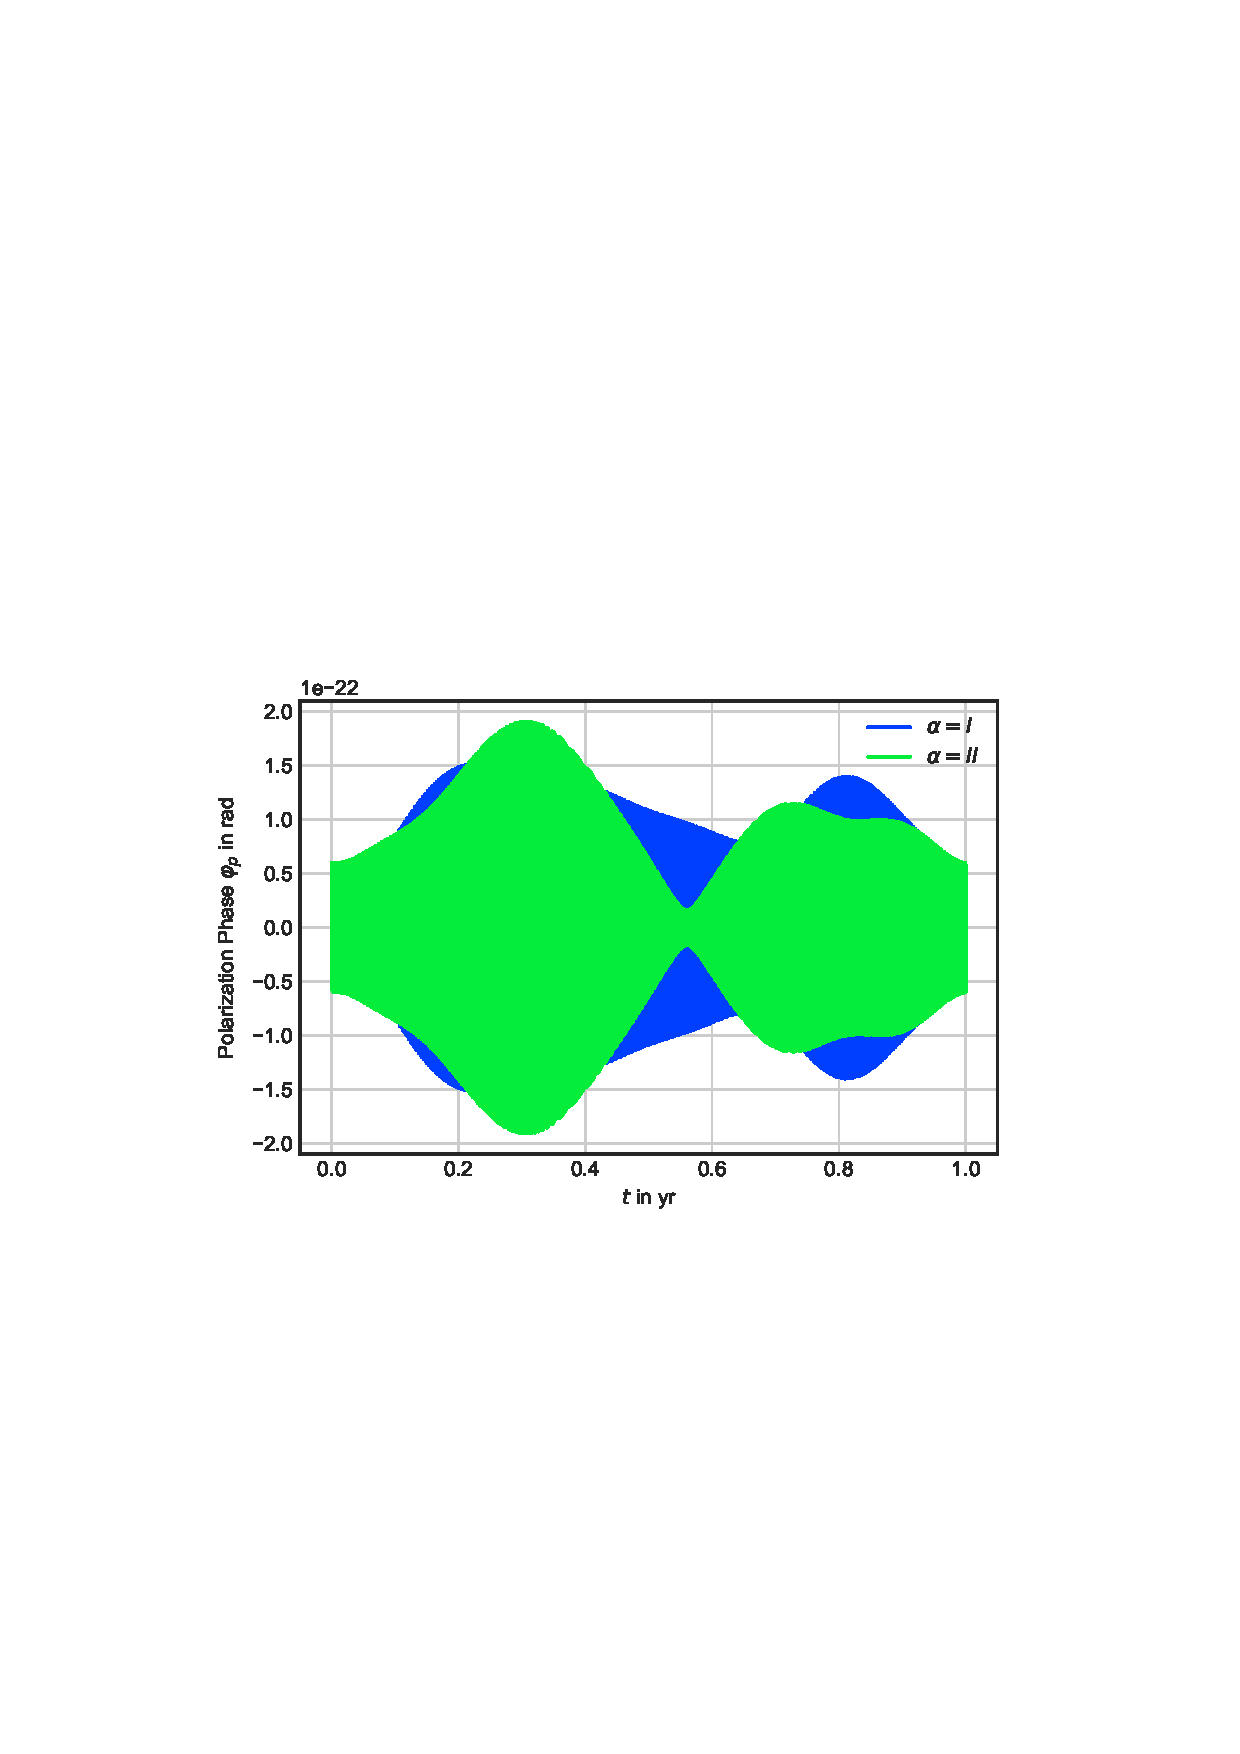
\includegraphics[width=.5\textwidth]{Strain.pdf}
\caption{The strain of a DWD binary over one year in LISA. The parameters are set as in \citep{cutler} at $\cos \theta_S = 0.3,\ \phi_S=5.0,\ \cos \theta_L = -0.2,\ \phi_S=4.0,\ f_0 =10\ \mathrm{mHz},\  M_1=M_2=0.23\ M_\odot$ and $r=1$ kpc. Note that the apparent filling is due to the $f_0 \times 1\ \mathrm{yr}\sim 316'000$ periods and the change in frequency is not resolvable although subsisting.}
    \label{fig:geometry}
\end{figure}

By determining the path of a source across LISA's field of vision, i.e. through $\theta_S(t),\ \phi_S(t),\text{ and }\psi_S(t)$ in its rest frame, we have finally arrived at the full parametric strain via eq.s \ref{eq:ampphase} through \ref{eq:endampphase}, and \ref{eq:FLISA}. The source path is given in \citep{cutler} through a series of equations.

The next step is to calculate the derivatives $\partial_i h(t,\lambda)$ for this strain. The first derivative is readily available, as

\begin{equation}
    \partial_{\mathrm{ln}(A)} h_\alpha(t) = h_\alpha(t).
\end{equation}

By focusing on eq.s \ref{eq:ampphase} through \ref{eq:endampphase}, and \ref{eq:phase}, we see that the parameters $\lambda=K,P,\varphi_0,f_0,\mathrm{ and }\ f_1$ enter only in $\Psi_\mathrm{obs}$ and $\varphi_D$ and therefore the derivative for these parameters is of the form

\begin{equation}
\begin{split}
    \partial_i h_\alpha (t) &= -\frac{\sqrt{3}}{2} \left( \partial_i \Psi_\mathrm{obs} + \left(\partial_i f\right) \frac{\varphi_D}{f(t)} \right) \\
    &\times A_\alpha(t)\sin \left(\Psi_\mathrm{obs}(t)+ \varphi_D(t) + \varphi_{p,\alpha}(t)\right),
\end{split}
\end{equation}

They can be calculated straightforwardly from eq. \ref{eq:freq} and \ref{eq:phase}, but we will state them anyways, as they will be used in Sec. \ref{sec:IG} as well

\begin{equation} \label{eq:derivsstart}
\begin{split}
    \partial_K f &= -\left((f_0+f_1 t) \cos \left(\frac{2 \pi  t}{P}+ \varphi_0 \right)\right)\\
    \partial_K \Psi_\mathrm{obs} &= \frac{P}{4\pi^2} \Bigg(-2 \pi  (f_0+f_1 t) \sin \left(\frac{2 \pi  t}{P}+\varphi_0\right) \\ &+2 \pi  f_0 \sin
   (\varphi_0)-f_1 P \cos \left(\frac{2 \pi  t}{P}+\varphi_0\right)+f_1 P \cos (\varphi_0) \Bigg)
\end{split}
\end{equation}
\begin{equation}
\begin{split}
    \partial_P f &= -\frac{2 \pi  K t (f_0+f_1 t) \sin \left(\frac{2 \pi  t}{P}+\varphi_0\right)}{P^2} \\
    \partial_P \Psi_\mathrm{obs} &= \frac{1}{2 \pi ^2 P} \Bigg( K \bigg(\left(2 \pi ^2 f_0 t-f_1 P^2+2 \pi ^2 f_1 t^2\right) \cos \left(\frac{2 \pi
   t}{P}+\varphi_0\right) \\ &+\pi  P \left(f_0 \sin (\varphi_0)-(f_0+2 f_1 t) \sin \left(\frac{2 \pi 
   t}{P}+\varphi_0\right)\right) \\&+f_1 P^2 \cos (\varphi_0)\bigg) \Bigg)
\end{split}
\end{equation}
\begin{equation}
\begin{split}
    \partial_{\varphi_0} f &= K (f_0+f_1 t) \sin \left(\frac{2 \pi  t}{P}+\varphi_0\right) \\
    \partial_{\varphi_0} \Psi_\mathrm{obs} &= \frac{K P}{4 \pi
   ^2}\Bigg( -2 \pi  (f_0+f_1 t) \cos \left(\frac{2 \pi  t}{P}+\varphi_0\right) \\ &+2 \pi  f_0 \cos
   (\varphi_0)+f_1 P \left(\sin \left(\frac{2 \pi  t}{P}+\varphi_0\right)-\sin (\varphi_0)\right) \Bigg)
\end{split}
\end{equation}
\begin{equation}
\begin{split}
    \partial_{f_0} f &= 1-K \cos \left(\frac{2 \pi  t}{P}+\varphi_0\right) \\
    \partial_{f_0} \Psi_\mathrm{obs} &= t-\frac{K P \sin \left(\frac{\pi  t}{P}\right) \cos \left(\frac{\pi  t}{P}+\varphi_0\right)}{\pi }
\end{split}
\end{equation}
\begin{equation} \label{eq:derivsend}
\begin{split}
    \partial_{f_1} f &= t \left(1-K \cos \left(\frac{2 \pi  t}{P}+\varphi_0\right)\right) \\
    \partial_{f_1} \Psi_\mathrm{obs} &= \frac{t^2}{2}-\frac{K P }{4 \pi ^2} \Bigg(2 \pi  t \sin \left(\frac{2 \pi  t}{P}+\varphi_0\right)\\&+P \cos \left(\frac{2 \pi 
   t}{P}+\varphi_0\right)-P \cos (\varphi_0)\Bigg)\,.
\end{split}
\end{equation}

The derivatives of the remaining positional parameters $\lambda=\theta_S,\phi_S,\theta_L$ and $\phi_L$ have in principle an analytical structure, but they are too long to be stated here and furthermore run slower than a simple numerical derivative, which we utilized in the end.

As the third ingredient remains only the strain sensitivity curve, which we took from \citep{Robson}. For a single mission however, we can generalize our results, such that they stay relevant even if the mission details and therefore the noise changes. For this we have to note, that in the derivation of the Fisher information matrix we found that $\Gamma \propto 1/S_n(f_0)$ due to the occurence of the inner product as defined in eq. \ref{eq:innerprod} for nearly monochromatic signals. 

\begin{figure}
    \centering
    \includegraphics[width=.5\textwidth]{Fisher_integrand.pdf}
    \caption{An example of the integrands to be used for the calculation of the Fisher information matrix in LISA, $\Gamma_{P\, \mathrm{ln}(A)}=\int_0^{T_\mathrm{obs}} \partial_P h_\alpha (t)\partial_{\mathrm{ln}(A)}(t) dt$ for a system with a $P=8.5$ yr CBP. Note that we can already see that the integral will be close to zero, as the two functions $\partial_i h_\alpha (t)$ do not appear to be in phase and oscillate around zero.}
    \label{fig:Fisher_ex}
\end{figure}

Evidently, the covariance matrix $\Sigma \propto S_n(f_0)$ and therefore the relative uncertainties, which are just the square root of the diagonal entries $\sigma_i=\sqrt{\Sigma_{ii}}\propto S_n(f_0)^{1/2}$. As similiarly the signal-to-noise scales as $S/N \propto S_n(f_0)^{-1/2}$, compare eq. \ref{eq:snr}, we can normalize our results with respect to signal-to-noise. Consequently, by stating the quantity $\sigma_i \cdot S/N$, we lose the dependance on strain sensitivity. This can be interpreted either as stating uncertainties for $S/N=1$ or in general as having to devide the quoted uncertainties by the $S/N$ of a given source to get the resulting uncertainty.

\subsection{Doppler Tracking}
\label{sec:IG}

For the proposed Doppler tracking mission, we have to repeat the same steps as with LISA, but will leave the inclusion of detailed orbits of the spacecrafts for future, more in-depth analysis. We want to shortly discuss the doppler tracking principle as reviewed in \citep{armstrong} and developed in \citep{estabrook}. 

Imagine a spacecraft being positioned at some distance in light-travel time $L=cT_2/2$ from earth. $T_2$ is in this case the two-way light time. Earth and the spacecraft act as free test masses and a ground station on earth continuously transmits a nearly monochromatic microwave signal centered at frequency $\nu_0$, which is coherently transponded by the distant spacecraft and sent back to earth. 

The ground station can then compare the received frequency to the emitted one at a time $t-T_2$ by monitoring the two-way fractional frequency fluctuation $y_2(t)=[ \nu_\mathrm{em}(t-T_2) -\nu_\mathrm{re}(t)]/\nu_0$. This way, the dimensionless velocity of the system $2\Delta v/c=\Delta \nu/\nu_0$ can be measured and should be $y_2\equiv 0$ in the absence of noise, systematic effects and of intercepting GWs, which may cause shifts of order $h$ in this observed quantity.

The strain of a GW from a source dircetion $n^a$ and with the earth-spacecraft direction $l^a$ will then be

\begin{equation} \label{eq:Doppler}
    y_2^{gw}(t) \equiv h(t) = \frac{\mu-1}{2} \Bar{\Psi}(t) - \mu \Bar{\Psi}\left(t-\frac{\mu+1}{2}T_2\right)+\frac{\mu+1}{2}\Bar{\Psi}(t-T_2)
\end{equation}
where $\mu=n^a l_a=\cos (i)$, $\Bar{\Psi}(t)=(h_{ab}(t)l^al^b)/(1-\mu^2)$ and $h_{ab}(t)$ as in eq. \ref{eq:GWtensor}, though with a general polarization basis and not necessarily the principal axes.

We find a `three-pulse' response of the system to a shock of gravitational radiation: One event due to buffeting of the earth by the GW, one event due to buffeting of the spacecraft a projected one-way light time later, and a third of the earth after the two-way light time. For long-wavelength events $f_0 \ll 1/T_2$ the waves partially cancel, but for the opposite limit, which is of interest to us, $T \ll T_2$, the full three-pulse character is present in the Doppler time series. As we focus our work on continuous GW emission, the waves will therefore interfere with themselves positively or negatively based on their characteristics.

As in \citep{soyuer2021}, we focus our analysis on a mission timeline for missions to Uranus and Neptune projected as
\begin{itemize}
    \item \textbf{Feb. 2031}: Space Launch System (SLS) departure from Aarth.
    \item \textbf{Dec. 2032}: Seperation of the spacecrafts and subsequent Jupiter Gravity Assist.
    \item \textbf{Apr. 2042}: Arrival of the first spacecraft on Uranus.
    \item \textbf{Sep. 2044}: Arrival of the second spacecraft at Neptune.
\end{itemize}

By assuming these time-stamps for the calculations of the trajectories under solar gravity and using intial velocities as stated after the proposed Jupiter Gravity Assist, it turns out that the spacecrafts spend most of their lifetime at a distance of $\sim 15$ AU and therefore with $T_2\approx 15'000$ s $\gg1$ h. They also enter near-conjunction $\varepsilon>150^\circ$ for $\sim 2$ month per year, which enables around ten 40-day observations through the radio link, as in near-conjunction noise by solar activity and irregularities in Earth's ionosphere is reduced fundamentally.

For our simplified model we therefore assume the spacecrafts at a fixed position at a two-way distance $T_2 = 15'000$ s and ten 40-day observations of the fractional frequency fluctuations in order to observe exoplanets around DWDs.

To arrive at the uncertainties of these measurements for an ice giant mission, we have to repeat the calculations of Sec \ref{sec:LISA} with eq. \ref{eq:Doppler}.

In heliocentric ecliptic coordinates, the coordinates of $l^a$ will be of the form $\theta_l\approx \pi/2$, $\phi_l$ and with the addition of source position $\theta_S,\ \phi_S$, we can compute $\mu$ easily by returning into cartesian coordinates to find with the short-hand $\Delta \phi = \phi_S-\phi_l$

\begin{equation}
    \mu = \cos (\Delta \phi) \sin (\theta_S).
\end{equation}

Next, in order to find $\Bar{\Psi}(t)$, we are interested in $h_{ab}(t)l^al^b$, which in comparison with eq. \ref{eq:beampattern} just turns out to be the beam-pattern function for a single arm of an interferometer $D^{ab}=l^al^b$. In the source frame $(p^a,q^a,n^a)$, we have the GW tensor given as in eq.s \ref{eq:preGWtensor} and \ref{eq:GWtensor}. In more explicit matrix notation this can be written as

\begin{equation}
    h_{ab}^{(S)} = 
    \begin{pmatrix}
    h_+ & h_\times & 0 \\
    h_\times & -h_+ & 0 \\
    0 & 0 & 0 \\
    \end{pmatrix}_{ab}
\end{equation}

Now the rotation, which brings the source frame into the $(l^a,y^a,z^a)$ detector frame, is given by a rotation by an angle $\theta_S$ around the y-axis, followed by a rotation by an angle $\Delta \phi$ around the x-axis

\begin{equation}
    \mathcal{R} = \begin{pmatrix}
\cos \Delta \phi & \sin \Delta \phi & 0 \\
-\sin \Delta \phi & \cos \Delta \phi & 0 \\
0 & 0 & 1 \\
\end{pmatrix}
\begin{pmatrix}
\cos \theta_S & 0 & \sin \theta_S\\
0 & 1 & 0 \\
-\sin \theta_S & 0 & \cos \theta_S
\end{pmatrix}
\end{equation}
and with the transformation law of the GW tensor, or just any 2-tensor in that sense, $h_{ab}=\mathcal{R}_{ac}\mathcal{R}_{bd}h_{cd}^{(S)}$, we can read off the necessary quantity $h_{ab}(t)l^al^b=h_{ll}$ in the detector frame

\begin{equation}
\begin{split}
    h_{ab}(t)l^al^b &= h_+(\cos^2 \theta_S \cos^2 \Delta \phi-\sin^2 \Delta \phi) \\ &+ h_\times 2(\cos \theta_S \sin \Delta \phi \cos \Delta \phi)
\end{split}
\end{equation}

As stated before, this can also be interpreted as the beam-pattern function of a one-way doppler tracking detector, which again can be rotated around the polarization basis by the polarization angle $\psi_S$ to express our result as  the amplitude-and-phase form. The beam pattern functions are in this model time-independent and read

\begin{equation}
\begin{split}
    F_+(\theta_S,\Delta \phi,\psi_S) &= (\cos^2 \theta_S \cos^2 \Delta \phi-\sin^2 \Delta \phi)\cos 2\psi_S \\
    &-2(\cos \theta_S \sin \Delta \phi \cos \Delta \phi)\sin 2\psi_S \\
    F_\times(\theta_S,\Delta \phi,\psi_S) &= (\cos^2 \theta_S \cos^2 \Delta \phi-\sin^2 \Delta \phi)\sin 2\psi_S \\
    &+2(\cos \theta_S \sin \Delta \phi \cos \Delta \phi)\cos 2\psi_S.
\end{split}
\end{equation}

And we result in

\begin{equation}
    \Bar{\Psi}(t) = \frac{A}{1-\mu^2} \cos \left(\Psi_\mathrm{obs} + \varphi_p \right)
\end{equation}
with $A, \varphi_p$ (without a time dependence) given as in eq.s \ref{eq:ampphase1} and \ref{eq:ampphase2}. As expected, the resulting strain will just be a phase-shifted and amplitude-modified superposition of the same wave three times.

Regarding the derivatives of the strain when completed in eq. \ref{eq:Doppler}, we again note, that the parameters $\lambda=K,P,\varphi_0,f_0,$ and $f_1$ enter only in $\Psi_\mathrm{obs}$, and therefore the derivatives from eq. \ref{eq:derivsstart} through \ref{eq:derivsend} can be repurposed in the general solution for $h(t)$ in a similar fashion as with LISA. The positional derivatives of the strain are again analytically performable but costly and we opted for numerical derivatives instead.

As the final ingredient we need to assume a strain sensitivity for an ice giant mission, which we quote from \citep{soyuer2021}. A compilation of Cassini-era noise sources are listed in \citep{armstrong} and the strain sensitivity can be modeled as a triple power-law, corresponding to three frequency regimes that are dominated by different noise sources as described by \citep{godtierpaper}

\begin{equation}
    S_n(f)=S_0 \sum_{i=1}^{3} \left( \frac{f}{f_i}\right)^{\alpha_i}
\end{equation}
where $f_1 < f_2 < f_3$ and $S_0$ is related to the so-called Allan deviation $\sigma_y$ via $S_0=T_2 \sigma_y^2$. For Cassini, the powers read $\alpha_1=-2,\alpha_2=-1/2,$ and $\alpha_3=2$, where the last two model the frequency propagation noise and the onset of thermal noise, respectively.

In our final computations we chose the DWD system parameters to be $\cos \theta_S = 0.3,\ \phi_S=5.0,\ \cos \theta_L = -0.2,\ \phi_S=4.0,\ f_0 =10\ \mathrm{mHz},\  M_1=M_2=0.23\ M_\odot$, $r=1$ kpc and $\phi_l=0$, which results in $\mu=0.27$ for a doppler tracking survey. We chose $f_0=10$ mHz, as LISA will detect DWDs with this frequency with high $S/N$. We further chose an edge-on CBP with inclination $i=\pi/2$, initial phase $\varphi_0=\pi/2$ and $M_P=10\ M_J$. The mass of the exoplanet turns out to be arbitrary to first order in our calculations however, as the relative uncertainties scale inversely to $K\propto M_P$ for $M_P \ll M_b$ as in our assumption of a CBP. This can be seen in the derivatives of eq.s \ref{eq:derivsstart} through \ref{eq:derivsend}: 

The derivatives $\partial_{P,\, \varphi_0} X(t) \propto K$ and $\partial_K X(t) \propto K^0$ with $X(t)=\Psi_\mathrm{obs}, f$. This results in a $\sigma^2_{P,\,\varphi_0}\propto K^{-2}$ after inversion of the (block) Fisher information matrix, and furthermore a $\sigma_K/K \propto K^{-1}$ after division by $K$. Due to this we quote the resulting uncertainties as $\sigma_\lambda/\lambda \cdot S/N \cdot M_P/M_J$ as with the signal-to-noise ratios.

\section{Results}
\label{sec:res}

Having compiled all the necessary equations, the final step is to compute the Fisher matrix for a nearly monochromatic signal by numerically performing the integration

\begin{equation} \label{eq:fisher}
    \Gamma_{ij} = \frac{2}{S_n(f_0)} \int_0^{T_\mathrm{obs}} \partial_i h(t) \partial_j h(t) dt.
\end{equation}

Then we can either inverse the Fisher information to recover the expected covariance matrix or add together Fisher information matrices of different detectors prior to inversion, to recover the total covariance recovered in a joint search. Note that for this step we need however information about the strain sensitivity $S_n(f)$, as we cannot add rescaled Fisher information matrices.

\begin{figure}
    \centering
    \includegraphics[width=.5\textwidth]{Relative_Uncertainties_l.pdf}
\caption{The rescaled LISA estimation of planetary parameters. The relative accuracy on $K$ and $P$ and absolute accuracy on $\varphi_0$ rescaled by $S/N$ and the CBPs mass measured in Jupiter masses. Crosses represent our computed uncertainties, solid lines serve as a reference taken from \citep{tamanini}. The GW frequency was set to $f_0=10$ mHz, and the position and angular momentum as in Tamanini & Danielski. Note the distinct features at higher orbital periods which are due to lower precision in the numerical integration due to computing constraints. The last data point at $P=10$ yr returned negative variances on the exoplanet parameters due to residual errors in the numerical integration and was left out, but may be interpreted as insensitivity towards exoplanets of $P\gtrsim 10$ yr.}
    \label{fig:LISA_res}
\end{figure}

We repeated the analysis for LISA as seen in Fig. \ref{fig:LISA_res}. The integrands are stated in Sec. \ref{sec:LISA} and we integrated numerically via Clenshaw–Curtis quadrature. We performed the integrals for each signal $\alpha=I,\, II$ separately and added the Fisher information matrices prior to inversion. 

The reason for our worse performance in comparison to Tamanini is due to a lack of computing power (or better adapted special-purpose integrators): In total, we need to compute two symmetric $9\times 9$ matrices (one per signal), so 90 integrals of expensive, oscillating functions of the type $A(t)\cos(\omega(t)t+\Phi_0) + B(t)$ with $\sim 316$ k periods and varying amplitudes via interpolation of Chebyshev polynomials, see Fig. \ref{fig:Fisher_ex} as an example. 

We opted for reasonable accuracy in our computations with relative errors of the integration of $1\%$ and a limit of 100 k sub divisions. This still resulted however in relative errors of up to 2'000\% for the more complicated integrands as the one shown in the figure, which may be further amplified by the non-linear matrix inversion. This was especially obvious in the occurrence of negative variances in the covariance matrix. We further tried weighted integrands and stratified Monte Carlo integration to no avail, as they did not display better convergence.

\begin{figure}
    \centering
    \includegraphics[width=.5\textwidth]{Tamanini_comp.pdf}
    \caption{The result for the reduced $3\times 3$ Fisher information approach for a binary at $f_0=10$ mHz, i.e. fixed source position, angular momentum and distance. Dashed lines represent the result for two ice giant missions with $\mu = 0.27$, triangles represent the reduced approach for all three arms of LISA. Solid lines denote the full parameter search taken from \citep{tamanini} as a reference.}
    \label{fig:comp_s}
\end{figure}

By reducing the parameter space or equivalently fixing the source position, angular momentum and separation, the one-year degeneracy for LISA's extraction of exoplanet parameters disappears completely and the relative uncertainties are reduced. In this case we only focus on the $3\times 3$ Fisher information matrix from the exoplanet parameters $\lambda=K,P,\varphi_0$. A comparison of LISA and an ice giant doppler tracking mission can be seen in Fig. \ref{fig:comp_s} for this simplified model. As expected, given that an ice giant mission can reach $S/N\gtrsim 1$, it would in fact be sensitive to CBPs with much longer periods compared to LISA.

Regarding the ice giant missions, we performed the same computation to arrive at the full $9 \times 9$ Fisher information matrix for one mission and multiplied the result by 2 in order to account for two measurements, but lost the dependance of our signal on the source location and orientation of the orbital plane in the process, as a single arm detector is incapable of determining the polarization state of an incident GW. 

Parameter independance of the signal however results in a singular Fisher matrix, which is not achievable with error-prone numerical integrations, as the set of singular matrices is a zero-set of the quadratic matrices because it is the inverse image of the continuous polynomial $\mathrm{det}^{-1}(0)$. Instead, we will find unphysical negative variances after the inversion, signaling an insensitivity on some of the parameters. This interpretation can also be chosen for the absence of the $P=10$ yr data point in LISA in Fig. \ref{fig:LISA_res}.

Accordingly, for an ice giant mission on its own we only state the results for the reduced $3\times 3$ Fisher matrix approach for an ice giant mission in Fig. \ref{fig:comp_s} and use the singular full parameter results for a joint search with LISA. As the ice giant mission is less computationally expensive, we could easily generate more data points.The variations of the relative uncertainties for $P<3$ yr is due to ice giant with its 40-day measurement once per year being quite sensitive to the initial phase and whether it can observe the amplitude of the doppler modulation or not. Additionally as expected minimal variances are returned for $P\approx 10$ yr, as the whole radial motion of the DWD due to the presence of a CBP can be resolved.

\begin{figure}
    \centering
    \includegraphics[width=.5\textwidth]{rel_uncertainty_added_10x.pdf}
    \caption{The resulting relative uncertainties by performing a joint ice giant doppler tracking and LISA search for exoplanets for a $f_0=10$ mHz binary. Crosses represent our result for LISA on its own, squares show the relative uncertainties for a joint search. We assumed a ratio $w=0.1$ for the joint search, i.e. LISA being 10 times more sensitive than the corresponding doppler tracking mission for the given binary.}
    \label{fig:joint}
\end{figure}

By adding the Fisher information prior to inversion, we can make distinct predictions for the raised precision by joining a CBP search of an ice giant mission and LISA. Additionally, the total signal-to-noise adds in quadrature, which will however be insignificant, as expected signal-to-noise ratios for a doppler tracking mission will be far lower than LISA's. By defining the weight

\begin{equation}
    w=\frac{S/N_\mathrm{Doppler}}{S/N_\mathrm{LISA}} < 1
\end{equation}

of the $S/N$ of a given source, we can quote our result independent of the improvement in Allan deviation. The total improvement in signal-to-noise will be 
\begin{equation}
    S/N_\mathrm{tot}=\sqrt{(1+w^2)}\ S/N_\mathrm{LISA}\approx \left(1+\frac{w^2}{2}\right)\ S/N_\mathrm{LISA}
\end{equation}

We can then use prior to inversion eq.s \ref{eq:snr} and \ref{eq:fisher} with the weight as defined above, which results in a total Fisher information matrix

\begin{equation}
\begin{split}
    \Gamma_\mathrm{tot} &= \Gamma_\mathrm{LISA} + \Gamma_\mathrm{Doppler} \\ &= \left( S/N_\mathrm{LISA} \right)^2 \frac{ \sum_{\alpha=I,II} \int \partial_i h_\alpha(t) \partial_j h_\alpha(t) dt}{ \sum_{\alpha=I,II} \int h_\alpha^2(t) dt} \\ &+ \left( w\times S/N_\mathrm{LISA} \right)^2 \frac{\int \partial_i h(t) \partial_j h(t) dt}{\int h^2(t) dt}
\end{split}
\end{equation}

We find, that an ice giant doppler tracking mission would already help constrain CBP parameters of interest for $w\gtrsim 10^{-2}$. In Fig. \ref{fig:joint}, we chose to depict $w=0.1$, which corresponds to an improvement in Allan deviation of 100. Note that for such high weights the negative variances that appeared in our computations for LISA on its own (see Fig. \ref{fig:LISA_res}) due to a lack of numerical precision disappear, as ice giant helps in constraining the exoplanet.

As the $S/N\sim\sqrt{T/S_n(f)}h_0$ with $h_0$ the effective amplitude of the strain, we see that for a $100\times$ lower $S_n^{(LISA)}(f)$ and as LISA takes measurements over 4 yr and ice giant over 400 d in total, $S/N_\mathrm{Doppler}\sim 0.05 \times S/N_\mathrm{LISA}$, so a weight $w\gtrsim 10^{-2}$ should in principle be achievable.

\section{Discussion}
\label{sec:disc}

As alluded to earlier, the bottleneck of our analysis is the computational cost of evaluating a single Fisher information matrix for LISA or an ice giant mission with its $45\times 2=90$ or $45\times 10=450$ respective integrals of oscillating integrands of the form $A(t)\cos(\omega(t)t+\Phi_0) + B(t)$ and in LISA's case $\sim 316$ k periods. By setting the Clenshaw–Curtis parameters to a pursued $1\%$ tolerance and 100 k sub divisions, computations on our Dell XPS 15 9750, with an 6-core 8th gen Core i7 CPU, took upwards of 40 hr per Fisher matrix for LISA and 5 hr for an ice giant mission.

In order to make more reliable predictions and faithfully recreate the work of \citep{tamanini}, supercomputing capabilities, or better adapted special-purpose integrators have to be used to lower the numerical errors in the Fisher information matrices prior to inversion. Additionally, one should bear in mind that round-off errors can appear when utilizing numerical derivatives as we did for the determination of the position and orientation of the orbital plane. 

As anticipated, an ice giant mission will be  sensitive to CBPs around DWDs with orbital periods of up to $P\approx 10$ yr, provided LISA tells them for what to look, although the sensitivity to CBPs with up to $P\sim 40$ yr as in Fig. \ref{fig:comp_s} has to be dismissed, as exactly fixing the source position is possible only for very few DWD systems where GW and EM observations with high signal-to-noise ratios are possible. Compare also the shifted insensitivity of LISA to upwards of $10$ yr in that simplified case.

Additionally, as pointed out in \citep{soyuer2021}, an ice giant doppler mission would only in the best-case of an improvement in Allan deviation of about 100 with respect to Cassini-era measurements be able to observe individual DWDs with $S/N > 1$. Evidently, the first term in the derivation of the Fisher information matrix, see eq. \ref{eq:pdf}, cannot be dismissed easily and may influence the final result. The observed change in frequency over 10 yr similarly has to be large enough, that it can be resolved by a fourier transform of the individual 40-day signals, i.e. $\Delta f > 1/40$ d $\approx 3\times 10^7$ Hz, which sets $M_P\ \gg 5\ M_\oplus$ for a 10 yr exoplanet in order for an ice giant mission to observe the change in frequency in the first place.

In future more in-depth analyses, the actual orbits of two ice giant missions should be included in the analysis for a more reasonable model. The actual $S/N$ of individual DWDs in an ice giant doppler tracking mission has to be included for improvements in Allan deviation by a given factor, to determine via Galactic population synthesis the increase in potentially detectable CBPs with long orbital periods in comparison to a single LISA mission. Additionally, with the help of an ice giant mission, long period CBPs around loud X-ray binary systems, like the planet candidate M51-ULS-1b \citep{X_ray_binary} around an O-class star and a stellar remnant, either black hole or neutron star, may be distingushable.

%\TD{discuss noise}
%Noise papers:
%\citet{godtierpaper}\citet{noise}
%\citet{plasma}
%\citet{tropo}
%\citet{antenna}
%\TD{How many exoplanets could they see together?}
%TD{Future work: Repeat analysis with higher computation power, add two spacecrafts with orbits, How many more, add allan deviation, discuss X-ray binary extragalactic}


\section{Conclusion}
\label{sec:conclusion}

We have in our work reviewed all necessary ingredients to constrain the parameter uncertainties for a joint search of LISA and two ice giant doppler tracking mission for CBPs around DWDs. We further explored these uncertainties for a chosen DWD system with GW frequency $f_0=10$ mHz and varying orbital periods $P$ of the CBP to show that an ice giant doppler tracking survey is sensitive to CBPs with longer orbital periods up to the nominal travel time of 10 yr, given that it is able to resolve loud DWDs with $S/N\gtrsim 1$.

Let us now return to our precursory assumptions in Sec. \ref{sec:spaceborne}, that the addition of an ice giant doppler mission may a) increase $S/N_\mathrm{tot}$, b) lower the selection function of LISA on its own in favor of CBPs with orbital periods of up to $P\approx10$ yr and c) help constrain planets with orbital periods close to an integer multiple of LISA's orbital period of one year. It turns out, that the addition of such a mission will not raise $S/N$ in any noticeable way. If a doppler tracking survey can be more than $1\%$ as sensitive as LISA however, it will indeed have an impact in constraining long period CBPs. The same holds for planets with orbital periods close to multiples of one-year, given the initial phase of the CBPs orbit $\varphi_0$ is tuned, such that ice giant can resolve the doppler shift in the first place. We note however, that our analysis has to be repeated with higher computational power and should only be seen as a proof of concept.

Still, as the addition of a noise robust radio transponder to an ice giant mission is a very cheap option, and with the possibility in mind, that Jupiter-like planets around DWDs may be observable in a joint search of LISA and such a mission, one should ask the question, why the long time of flight should not be used in this fashion?

%\TD{If LISA tells ice giant where to look, it can help with long period exoplanets and potentially find a P-type Jupiter?}

%\TD{discuss potential X-ray binary extragalactic exoplanet detection}



\begin{acknowledgements}
We want to thank Kilian and Arman for enduring me complaining when my code didn't work, and the flat at Cäsar-Ritz-Strasse 7 for persevering my loud, hard-working Laptop in the living room every night. We also want to thank Amina for forcing me to stay at home and finish this report.
\end{acknowledgements}

% WARNING
%-------------------------------------------------------------------
% Please note that we have included the references to the file aa.dem in
% order to compile it, but we ask you to:
%
% - use BibTeX with the regular commands:
%   \bibliographystyle{aa} % style aa.bst
%   \bibliography{Yourfile} % your references Yourfile.bib
%
% - join the .bib files when you upload your source files
%-------------------------------------------------------------------

\bibliographystyle{aa}
\bibliography{biblio.bib}

\end{document}
%